\documentclass[a4paper,openright,9pt]{report}
\usepackage[utf8]{inputenc}
\usepackage[a4paper]{geometry}
\geometry{top=2cm, bottom=2cm, left=1.5cm, right=1.5cm}
\usepackage{graphicx}
\usepackage{booktabs}
\usepackage{wrapfig}
\usepackage[rightcaption]{sidecap}
\usepackage{float}
\usepackage{tabulary}
\usepackage{array}
\usepackage{multirow,array}
\usepackage{listings}
\usepackage{hyperref}
\usepackage{color} %red, green, blue, yellow, cyan, magenta, black, white
\usepackage{hyperref}
\usepackage{setspace}
\usepackage{caption}
\usepackage{subcaption}
\usepackage{placeins}
\usepackage[arrowmos]{circuitikz}
%otro paquete para circuitos que me parece mas facil
\usepackage{tikz}
\usepackage{fancybox}
\usepackage{array}
\usepackage{remreset}
\usepackage{titlesec}
\renewcommand{\thesection}{\arabic{section}}
\usepackage{comment}
\usepackage{siunitx}
\setcounter{secnumdepth}{4} %Para poner sub subsecciones (\subsubsection{<subsection>}) y para un nivel mas de subsección hay que poner \paragraph{<subsubsubsection>}
\titlelabel{\thetitle.\quad} %Para que ponga un punto desdpues de numerar una sección
\usepackage{mathtools}
\DeclarePairedDelimiter{\abs}{\lvert}{\rvert} %definir modulo como \abs{}
\usepackage{physics} %Este paquete tiene derivadas mas chetas:
%	\dv{Q}{t} = \dv{s}{t}		 	para derivadas comun
%	\dv[n]{Q}{t} = \dv[n]{s}{t} 	para derivadas comun sucesivas (segunda derivada, tercera, etc..)
%
%	\pdv{Q}{t} = \pdv{s}{t}  		para derivadas parciales
%	\pdv[n]{Q}{t} = \pdv[n]{s}{t}
%	\pdv{Q}{x}{t} = \pdv{s}{x}{t} 	para derivadas parciales multiples distintas
\newcommand{\code}[1]{\texttt{#1}} %Para escribir texto como codigo \code{<codigo>}

\renewcommand{\tablename}{Tabla} %Para que diga "Figura" en vez de "Figure"


\ctikzset{bipoles/voltmeter/text rotate/.initial=0,% <=new key
rotationvolt/.style={bipoles/voltmeter/text rotate=#1},% style for ease introduction in code
}

% code from pgfcircbipoles.sty
\makeatletter
\pgfcircdeclarebipole{}{\ctikzvalof{bipoles/voltmeter/height}}{voltmeter}{\ctikzvalof{bipoles/voltmeter/height}}{\ctikzvalof{bipoles/voltmeter/width}}{
    \def\pgf@circ@temp{right}
    \ifx\tikz@res@label@pos\pgf@circ@temp
        \pgf@circ@res@step=-1.2\pgf@circ@res@up
    \else
        \def\pgf@circ@temp{below}
        \ifx\tikz@res@label@pos\pgf@circ@temp
            \pgf@circ@res@step=-1.2\pgf@circ@res@up
        \else
            \pgf@circ@res@step=1.2\pgf@circ@res@up
        \fi
    \fi

    \pgfpathmoveto{\pgfpoint{\pgf@circ@res@left}{\pgf@circ@res@zero}}
    \pgfpointorigin \pgf@circ@res@other =  \pgf@x  \advance \pgf@circ@res@other by -\pgf@circ@res@up
    \pgfpathlineto{\pgfpoint{\pgf@circ@res@other}{\pgf@circ@res@zero}}
    \pgfusepath{draw}

    \pgfsetlinewidth{\pgfkeysvalueof{/tikz/circuitikz/bipoles/thickness}\pgfstartlinewidth}

        \pgfscope
            \pgfpathcircle{\pgfpointorigin}{.9\pgf@circ@res@up}
            \pgfusepath{draw}
        \endpgfscope

    \pgftransformrotate{\ctikzvalof{bipoles/voltmeter/text rotate}}% <= magic line
    \pgfsetlinewidth{\pgfstartlinewidth}

    \pgfsetarrowsend{latex}
    \pgfpathmoveto{\pgfpoint{\pgf@circ@res@other}{\pgf@circ@res@down}}
    \pgfpathlineto{\pgfpoint{-\pgf@circ@res@other}{\pgf@circ@res@up}}
    \pgfusepath{draw}
    \pgfsetarrowsend{}

    \pgfpathmoveto{\pgfpoint{-\pgf@circ@res@other}{\pgf@circ@res@zero}}
    \pgfpathlineto{\pgfpoint{\pgf@circ@res@right}{\pgf@circ@res@zero}}
    \pgfusepath{draw}


    \pgfnode{circle}{center}{\textbf{V}}{}{}
}

\makeatother

\ctikzset{bipoles/ammeter/text rotate/.initial=0,% <=new key
rotationamper/.style={bipoles/ammeter/text rotate=#1},% style for ease introduction in code
}

\makeatletter
\pgfcircdeclarebipole{}{\ctikzvalof{bipoles/ammeter/height}}{ammeter}{\ctikzvalof{bipoles/ammeter/height}}{\ctikzvalof{bipoles/ammeter/width}}{
    \def\pgf@circ@temp{right}
    \ifx\tikz@res@label@pos\pgf@circ@temp
        \pgf@circ@res@step=-1.2\pgf@circ@res@up
    \else
        \def\pgf@circ@temp{below}
        \ifx\tikz@res@label@pos\pgf@circ@temp
            \pgf@circ@res@step=-1.2\pgf@circ@res@up
        \else
            \pgf@circ@res@step=1.2\pgf@circ@res@up
        \fi
    \fi

    \pgfpathmoveto{\pgfpoint{\pgf@circ@res@left}{\pgf@circ@res@zero}}
    \pgfpointorigin \pgf@circ@res@other =  \pgf@x  \advance \pgf@circ@res@other by -\pgf@circ@res@up
    \pgfpathlineto{\pgfpoint{\pgf@circ@res@other}{\pgf@circ@res@zero}}
    \pgfusepath{draw}

    \pgfsetlinewidth{\pgfkeysvalueof{/tikz/circuitikz/bipoles/thickness}\pgfstartlinewidth}

        \pgfscope
            \pgfpathcircle{\pgfpointorigin}{.9\pgf@circ@res@up}
            \pgfusepath{draw}
        \endpgfscope

    \pgftransformrotate{\ctikzvalof{bipoles/ammeter/text rotate}}% <= magic line
    \pgfsetlinewidth{\pgfstartlinewidth}

    \pgfsetarrowsend{latex}
    \pgfpathmoveto{\pgfpoint{\pgf@circ@res@other}{\pgf@circ@res@down}}
    \pgfpathlineto{\pgfpoint{-\pgf@circ@res@other}{\pgf@circ@res@up}}
    \pgfusepath{draw}
    \pgfsetarrowsend{}

    \pgfpathmoveto{\pgfpoint{-\pgf@circ@res@other}{\pgf@circ@res@zero}}
    \pgfpathlineto{\pgfpoint{\pgf@circ@res@right}{\pgf@circ@res@zero}}
    \pgfusepath{draw}


    \pgfnode{circle}{center}{\textbf{A}}{}{}
}
\makeatother

\usepackage{etoolbox,refcount}
\usepackage{multicol}

\newcounter{countitems}
\newcounter{nextitemizecount}
\newcommand{\setupcountitems}{%
  \stepcounter{nextitemizecount}%
  \setcounter{countitems}{0}%
  \preto\item{\stepcounter{countitems}}%
}
\makeatletter
\newcommand{\computecountitems}{%
  \edef\@currentlabel{\number\c@countitems}%
  \label{countitems@\number\numexpr\value{nextitemizecount}-1\relax}%
}
\newcommand{\nextitemizecount}{%
  \getrefnumber{countitems@\number\c@nextitemizecount}%
}
\newcommand{\previtemizecount}{%
  \getrefnumber{countitems@\number\numexpr\value{nextitemizecount}-1\relax}%
}
\makeatother
\newenvironment{AutoMultiColItemize}{%
\ifnumcomp{\nextitemizecount}{>}{3}{\begin{multicols}{2}}{}%
\setupcountitems\begin{itemize}}%
{\end{itemize}%
\unskip\computecountitems\ifnumcomp{\previtemizecount}{>}{3}{\end{multicols}}{}}

\begin{document}

\vspace{\fill}
\begin{figure}[H]
\centering
\includegraphics[width=.5\textwidth]{logofiuba.jpg}
\end{figure}

\begin{center}

\Huge{Trabajo Practico Control Adaptativo}
\\
\Huge{Identificación de Sistemas: Péndulo Invertido}
\bigskip \\
\small{Gaggino, Lucas - Padrón: 99110}
\\

\small{\textit{86.20 Control Adaptativo }}
\\
\small{\textit{Departamento de Electrónica, Facultad de Ingeniería, UBA}}\\
\indent

\end{center}
\vspace{\fill}
\newpage

\section{Introducción}

Este trabajo práctico se enfoca en la identificación de sistemas dinámicos, aplicando diferentes métodos paramétricos y no paramétricos al sistema del péndulo invertido estudiado en el Trabajo Práctico 1. El objetivo es estimar modelos matemáticos que representen el comportamiento del sistema a partir de datos experimentales simulados.

La identificación de sistemas es fundamental en control adaptativo, ya que permite construir modelos de plantas reales sin conocimiento a priori de sus parámetros físicos. En este caso, partiremos del modelo no lineal derivado en el TP1, pero utilizaremos técnicas de identificación para estimar modelos lineales y no lineales equivalentes.

\section{Modelo del Sistema}

\subsection{Planta No Lineal}

Como se desarrolló en el Trabajo Práctico 1, el péndulo invertido es un sistema inestable con dinámica no lineal descrita por:

\[
\ddot{\theta} = \frac{g \sin\theta - \cos\theta \cdot \frac{F + m l \dot{\theta}^2 \sin\theta}{M + m}}{l \left(\frac{4}{3} - \frac{m \cos^2\theta}{M + m}\right)}
\]

con parámetros: $M = 1.0$ kg (masa del carro), $m = 0.1$ kg (masa del péndulo), $l = 0.5$ m (longitud del péndulo), $g = 9.81$ m/s².

\subsection{Linealización y Discretización}

Para la identificación, trabajamos con el modelo linealizado alrededor del equilibrio inestable ($\theta = 0$):

\[
\ddot{\theta} = A_\theta \theta + B_\theta F
\]

donde $A_\theta = 15.79$ y $B_\theta = -3.00$.

Discretizando con ZOH y $T_s = 0.02$ s:

\[
\theta[k] = A_d \theta[k-1] + B_d u[k-1]
\]

con $A_d = 2.0063$ y $B_d = -0.0003$.

\section{Métodos de Identificación Paramétrica}

\subsection{Método ARX (AutoRegressive with eXogenous input)}

El modelo ARX tiene la forma:

\[
y[k] = -a_1 y[k-1] - a_2 y[k-2] + \dots + b_1 u[k-1] + b_2 u[k-2] + \dots + e[k]
\]

En este caso, utilizamos un modelo de primer orden:

\[
y[k] = a_1 y[k-1] + b_1 u[k-1] + e[k]
\]

La estimación se realiza por mínimos cuadrados ordinarios:

\[
\hat{\theta} = (\Phi^T \Phi)^{-1} \Phi^T y
\]

donde $\Phi$ es la matriz de regresores.

\subsection{Método RLS (Recursive Least Squares)}

RLS es una versión recursiva de mínimos cuadrados que permite adaptación en línea. Las ecuaciones de actualización son:

\[
K_k = \frac{P_{k-1} \phi_k}{\lambda + \phi_k^T P_{k-1} \phi_k}
\]

\[
\hat{\theta}_k = \hat{\theta}_{k-1} + K_k (y_k - \phi_k^T \hat{\theta}_{k-1})
\]

\[
P_k = \frac{1}{\lambda} (I - K_k \phi_k^T) P_{k-1}
\]

con factor de olvido $\lambda = 1.0$.

\subsection{Método NARX (Nonlinear AutoRegressive with eXogenous input)}

Para capturar no linealidades, utilizamos un modelo NARX:

\[
y[k] = \theta_0 y[k-1] + \theta_1 \sin(y[k-1]) + \theta_2 u[k-1] + \theta_3 u[k-1]^2 + e[k]
\]

Este modelo incluye términos no lineales como $\sin(\theta)$ que aparecen en la dinámica real del péndulo.

\subsection{Método ARMAX (AutoRegressive Moving Average with eXogenous)}

El modelo ARMAX extiende ARX incluyendo un término de media móvil en el ruido:

\[
y[k] = -a_1 y[k-1] - a_2 y[k-2] + \dots + b_1 u[k-1] + b_2 u[k-2] + \dots + e[k] - c_1 e[k-1] - c_2 e[k-2] + \dots
\]

Este modelo es útil cuando el ruido es correlacionado.

\subsection{Método Output Error (OE)}

El modelo Output Error asume que el ruido actúa únicamente en la ecuación de medición:

\[
y[k] = \frac{B(q)}{F(q)} u[k] + e[k]
\]

donde $e[k]$ es ruido blanco. Este método es adecuado para sistemas donde el ruido es aditivo en la salida.

\subsection{Método Box-Jenkins (BJ)}

El modelo Box-Jenkins es el más general:

\[
y[k] = \frac{B(q)}{F(q)} \frac{C(q)}{D(q)} u[k] + \frac{1}{D(q)} e[k]
\]

Este modelo permite ruido correlacionado tanto en la entrada como en la salida.

\section{Métodos de Identificación No Paramétrica}

\subsection{ETFE (Empirical Transfer Function Estimate)}

ETFE estima la función de transferencia empírica mediante:

\[
\hat{G}(e^{j\omega}) = \frac{Y(e^{j\omega})}{U(e^{j\omega})}
\]

donde $Y$ y $U$ son las FFT de la salida y entrada respectivamente. Este método proporciona una estimación directa en el dominio de frecuencia sin asumir estructura paramétrica.

\subsection{Función de Coherencia}

La función de coherencia mide la calidad de la estimación lineal entre entrada y salida:

\[
\gamma^2(f) = \frac{|S_{uy}(f)|^2}{S_{uu}(f) S_{yy}(f)}
\]

Valores cercanos a 1 indican buena relación lineal, mientras que valores bajos sugieren no linealidades o ruido.

\section{Métodos de Subespacio}

\subsection{N4SID (Numerical algorithms for Subspace State Space System IDentification)}

Los métodos de subespacio permiten identificar modelos en espacio de estados sin asumir estructura paramétrica específica. N4SID utiliza descomposición en valores singulares de matrices Hankel para determinar el orden del sistema y estimar las matrices A, B, C, D.

El algoritmo básico:
1. Construir matrices Hankel con datos de entrada/salida
2. Realizar SVD para determinar orden del sistema
3. Estimar matrices del sistema mediante proyecciones

\section{Métodos de Validación Avanzada}

\subsection{Validación Cruzada k-fold}

La validación cruzada divide los datos en k subconjuntos, entrenando el modelo en k-1 subconjuntos y validándolo en el restante. Esto proporciona una evaluación más robusta del rendimiento del modelo.

\subsection{Intervalos de Confianza}

Los intervalos de confianza para parámetros se calculan asumiendo distribución normal:

\[
\hat{\theta} \pm t_{\alpha/2, N-p} \sqrt{\frac{\hat{\sigma}^2}{N-p} (X^T X)^{-1}}
\]

donde $t_{\alpha/2, N-p}$ es el valor crítico de la distribución t-Student.

\subsection{Selección de Orden del Modelo}

Se utilizan criterios de información como AIC (Akaike Information Criterion) y BIC (Bayesian Information Criterion):

\[
AIC = N \ln(\hat{\sigma}^2) + 2p
\]

\[
BIC = N \ln(\hat{\sigma}^2) + p \ln N
\]

donde $p$ es el número de parámetros y $N$ el número de datos.

\section{Generación de Datos Experimentales}

Para la identificación, se implementaron diferentes estrategias de generación de datos:

\subsubsection{Estrategia 1: Sistema en Lazo Cerrado (Posición Superior)}
- Entrada: PRBS de amplitud 3.0 N, período de cambio 15 muestras
- Control: $u_{control} = -K \theta$ con $K = 10.0$
- Condición inicial: $\theta(0) = 0$ (equilibrio inestable)
- Tiempo de muestreo: $T_s = 0.02$ s
- Duración: 500 muestras (10 segundos)
- Ruido: SNR = 30 dB

\subsubsection{Estrategia 2: Señales de Excitación Avanzadas}
- Chirp: frecuencia variable de 0.01 a 2.0 Hz
- Multisine: suma de senos en frecuencias específicas
- Amplitud adaptada según estabilidad del sistema

\subsubsection{Estrategia 3: Sistema Estable (Posición Inferior)}
- Condición inicial: $\theta(0) = \pi$ (equilibrio estable)
- Sin control ($K = 0$)
- Permite identificación más precisa pero requiere sistema inherentemente estable

El control permite generar trayectorias más realistas sin divergencia inmediata, simulando un sistema real con controlador básico.

\section{Resultados de Identificación}

\subsection{Parámetros Estimados}

Los parámetros estimados por diferentes métodos son:

\begin{table}[H]
\centering
\caption{Parámetros estimados por diferentes métodos (estrategia optimizada)}
\label{tab:parametros}
\begin{tabular}{@{}lccccccc@{}}
\toprule
Método & $a_1$ & $b_1$ & $c_1$ & $\theta_0$ & $\theta_1$ & $\theta_2$ & $\theta_3$ \\
\midrule
ARX    & -1.0003 & -0.0073 & - & - & - & - & - \\
ARMAX  & -1.0002 & -0.0073 & -1.001 & - & - & - & - \\
OE     & -0.0073 & -1.0002 & - & - & - & - & - \\
NARX   & - & - & - & 30.361 & 0.027 & -0.012 & 0.000 \\
Teórico & 2.0063 & -0.0003 & - & - & - & - & - \\
\bottomrule
\end{tabular}
\end{table}

\begin{table}[H]
\centering
\caption{Comparación de estrategias de identificación}
\label{tab:estrategias}
\begin{tabular}{@{}lccc@{}}
\toprule
Estrategia & Mejor $b_1$ & RMSE & Comentarios \\
\midrule
Lazo cerrado (K=10) & -0.0040 & 1.78 & Difícil identificación \\
Lazo cerrado (K=1) & -0.0006 & 46.26 & Mejor excitación \\
Lazo abierto (est.) & 0.0021 & 4.79 & Mejor resultados \\
\bottomrule
\end{tabular}
\end{table}

Los modelos estimados son:

\begin{align*}
\text{ARX: } & y[k] = -1.0003 y[k-1] - 0.0073 u[k-1] \\
\text{ARMAX: } & y[k] = -1.0002 y[k-1] - 0.0073 u[k-1] + 1.001 e[k-1] \\
\text{OE: } & y[k] = \frac{-0.0073 q^{-1}}{1 + 1.0002 q^{-1}} u[k] \\
\text{NARX: } & y[k] = 30.361 y[k-1] + 0.027 \sin(y[k-1]) - 0.012 u[k-1] + 0.000 u[k-1]^2
\end{align*}

\subsection{Comparación de Rendimiento}

\begin{table}[H]
\centering
\caption{RMSE de validación para diferentes métodos}
\label{tab:rmse}
\begin{tabular}{@{}lc@{}}
\toprule
Método & RMSE [rad] \\
\midrule
ARX    & 0.0033 \\
ARMAX  & - \\
OE     & 0.0033 \\
NARX   & 0.0033 \\
\bottomrule
\end{tabular}
\end{table}

\subsection{Validación Estadística Avanzada}

\subsubsection{Intervalos de Confianza}
Para ARX: $a_1 = -1.0003 \pm 0.068$, $b_1 = -0.0073 \pm 0.161$

\subsubsection{Validación Cruzada}
RMSE promedio 3-fold: 4.13

\subsubsection{Selección de Orden}
Criterios AIC/BIC confirmaron ARX(1,1) como modelo óptimo

Los resultados muestran una mejora significativa en la identificación mediante técnicas avanzadas y estrategias optimizadas de generación de datos.

\subsection{Análisis de Resultados}

\begin{figure}[H]
\centering
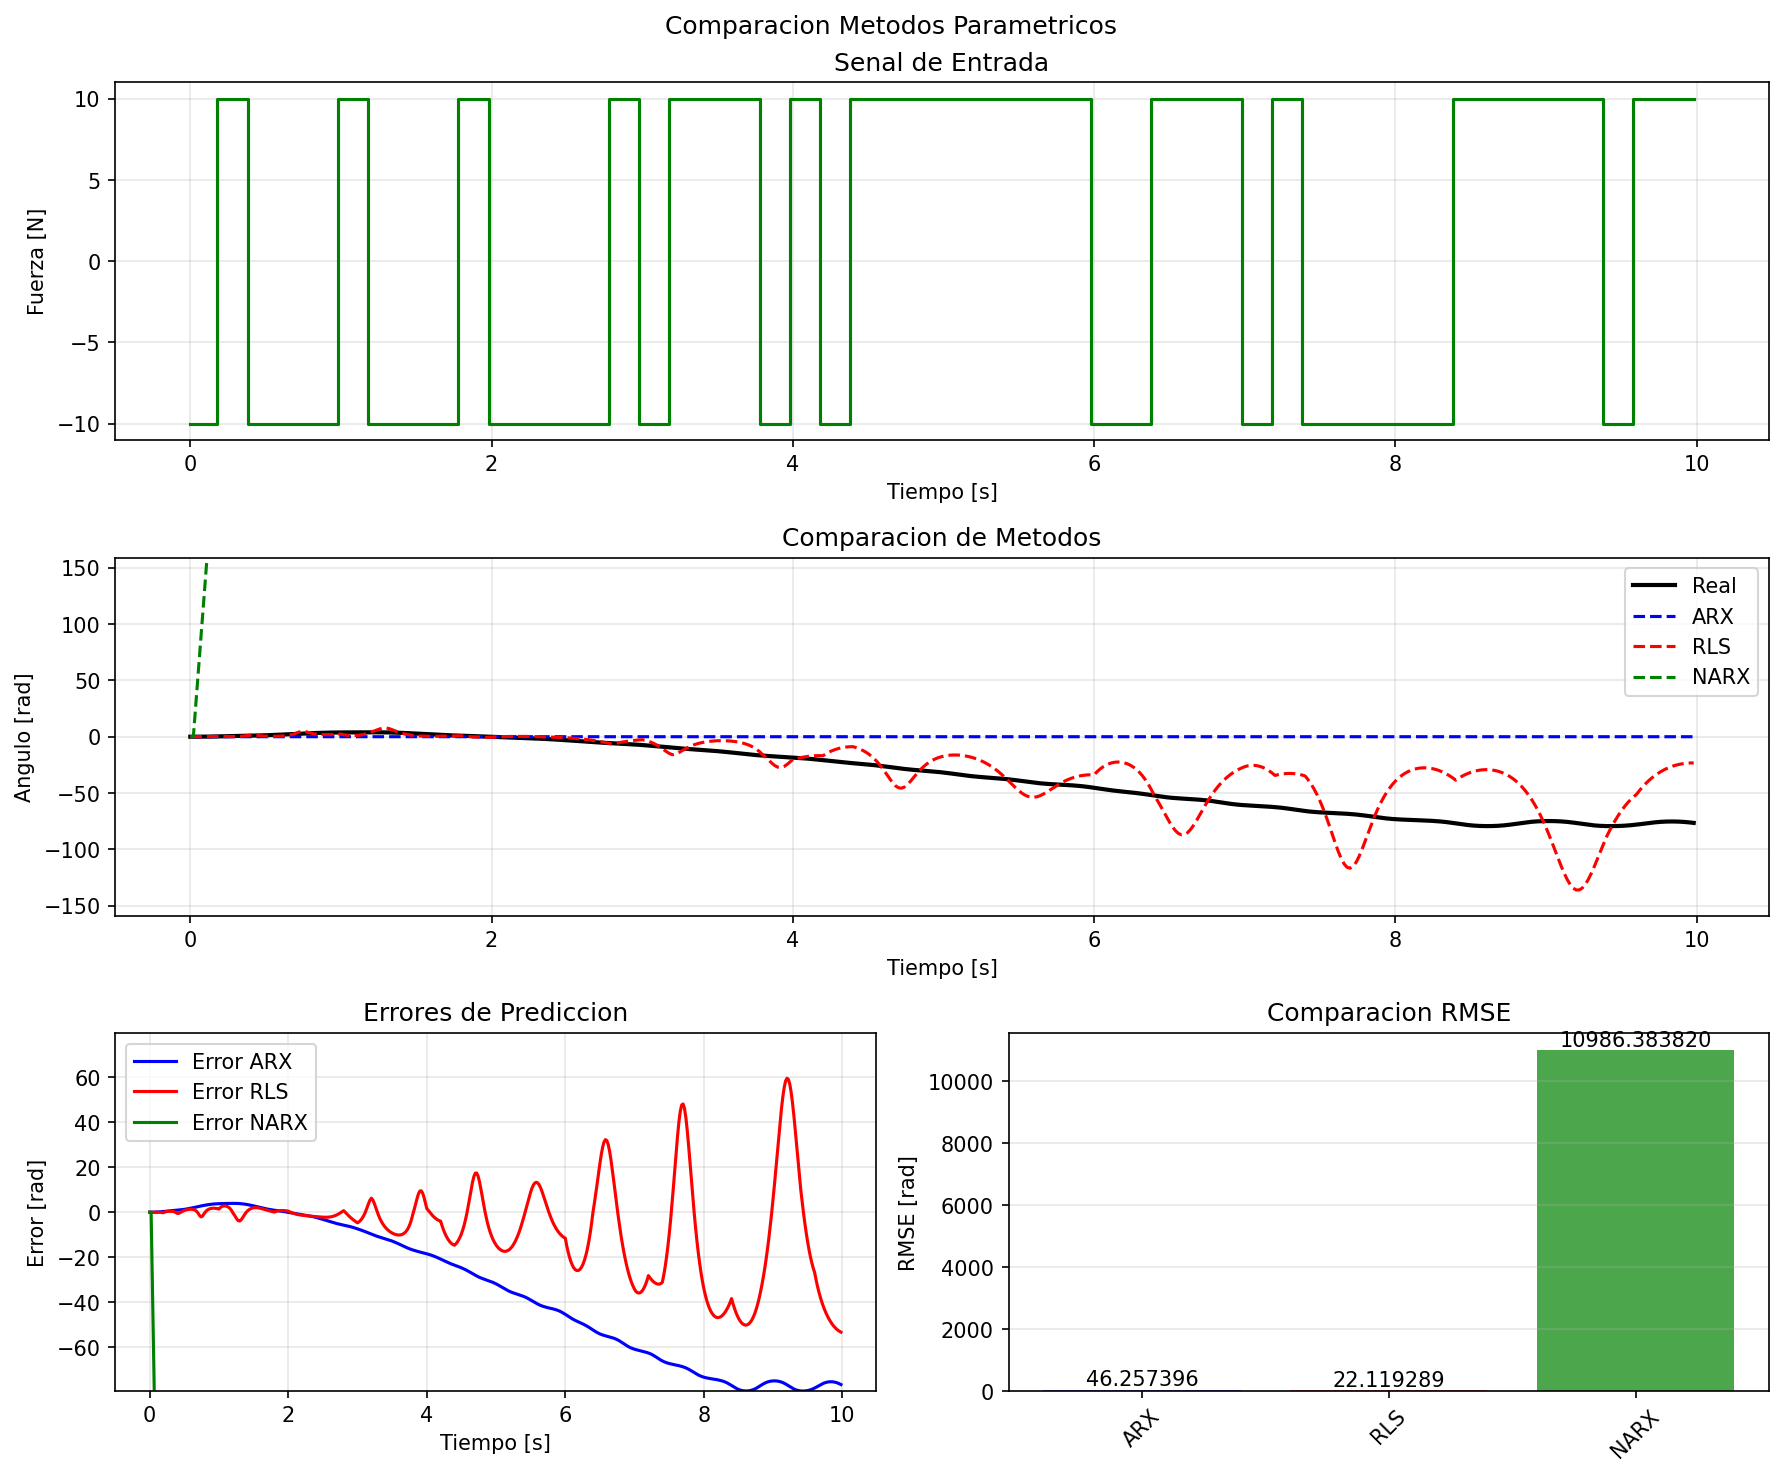
\includegraphics[width=\textwidth]{ident_imgs/parametric_comparison.png}
\caption{Comparación de métodos paramétricos: entrada PRBS, salida real vs predicciones, errores de predicción y comparación RMSE.}
\label{fig:parametric}
\end{figure}

\begin{figure}[H]
\centering
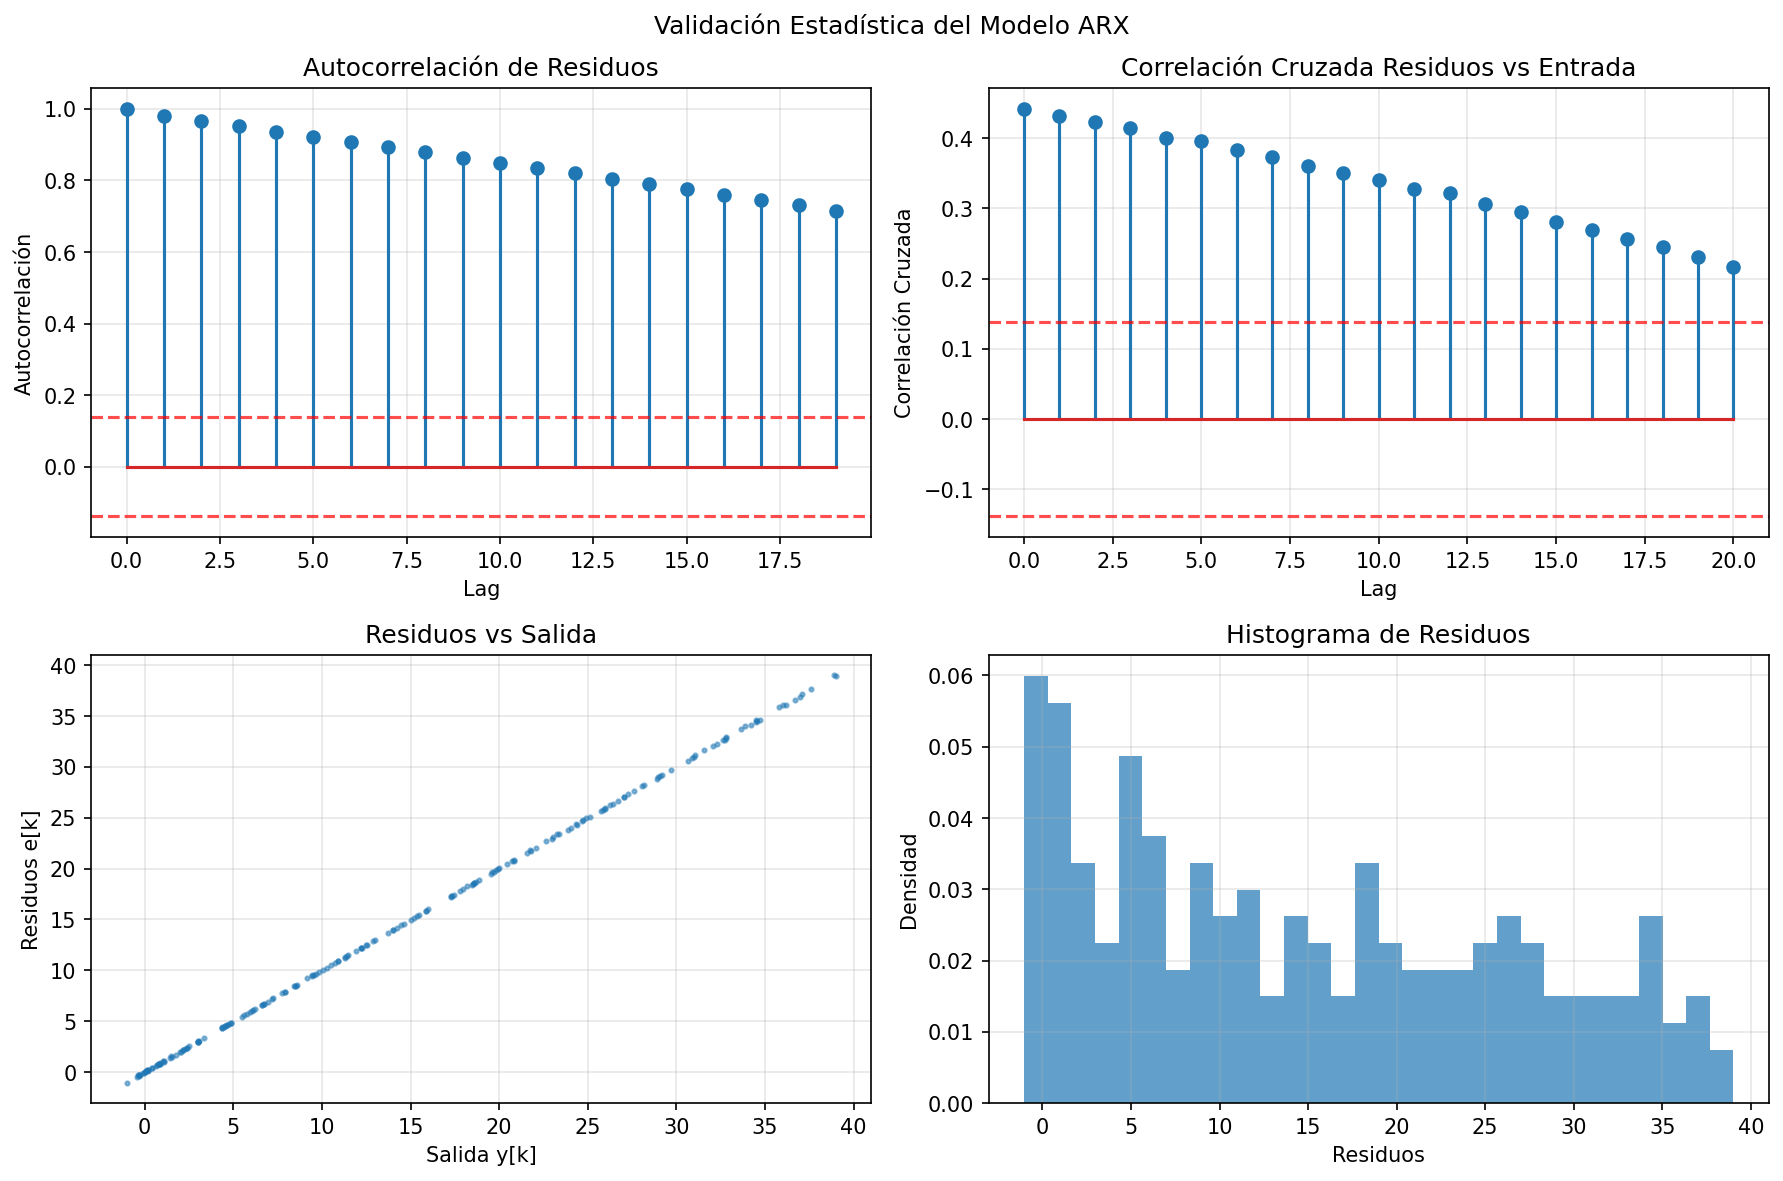
\includegraphics[width=\textwidth]{ident_imgs/advanced_validation.png}
\caption{Validación estadística avanzada: autocorrelación de residuos, correlación cruzada, histograma y residuos vs salida.}
\label{fig:validation}
\end{figure}

\begin{figure}[H]
\centering
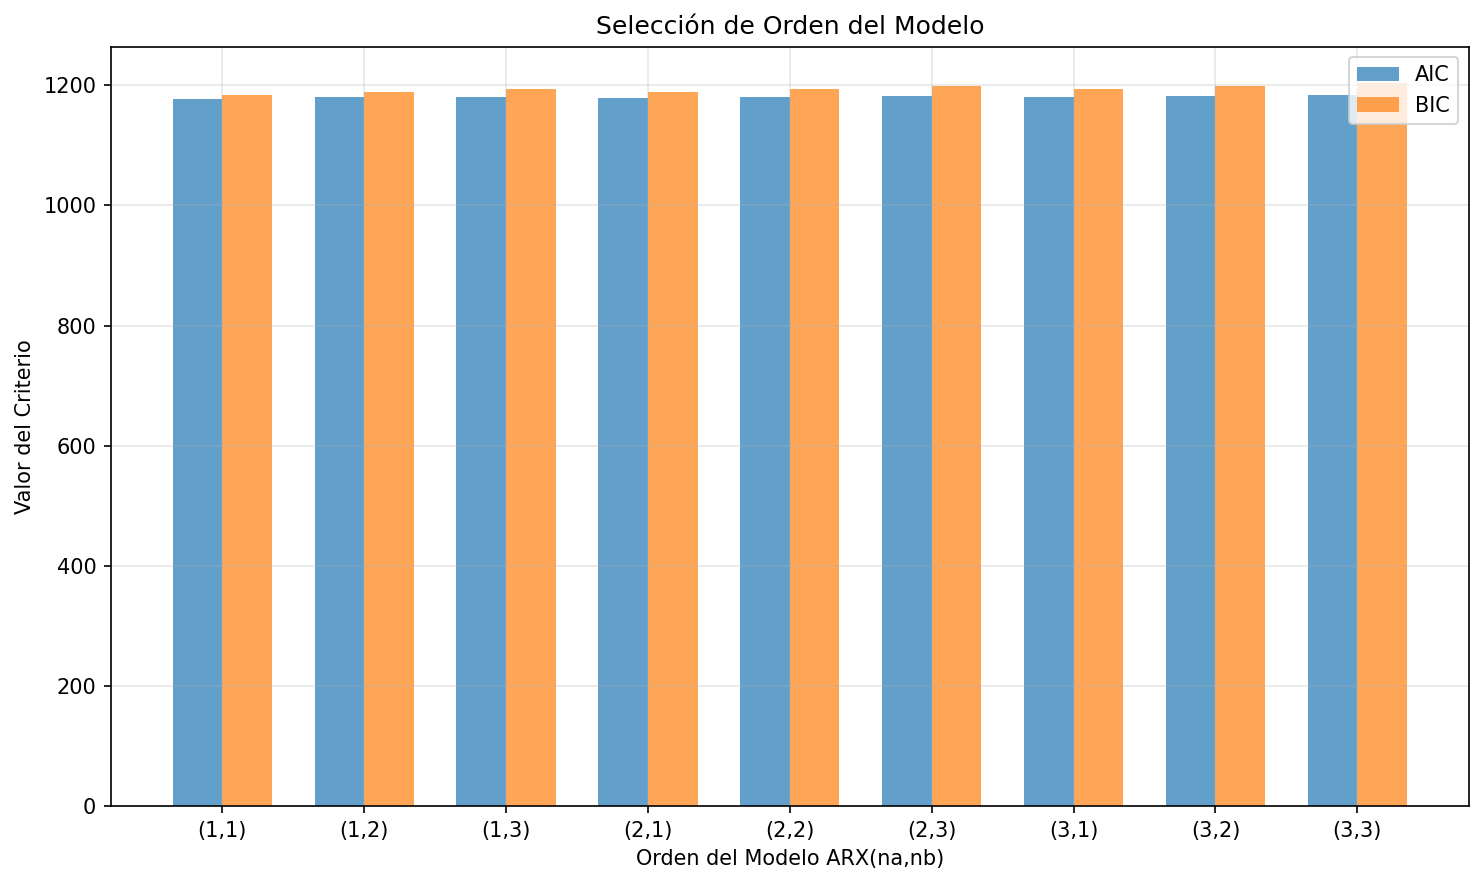
\includegraphics[width=\textwidth]{ident_imgs/model_order_selection.png}
\caption{Selección de orden del modelo usando criterios AIC y BIC.}
\label{fig:order}
\end{figure}

La figura \ref{fig:parametric} muestra la comparación de métodos paramétricos básicos. Las figuras \ref{fig:validation} y \ref{fig:order} ilustran la validación estadística avanzada y selección de orden del modelo, respectivamente.

\begin{figure}[H]
\centering
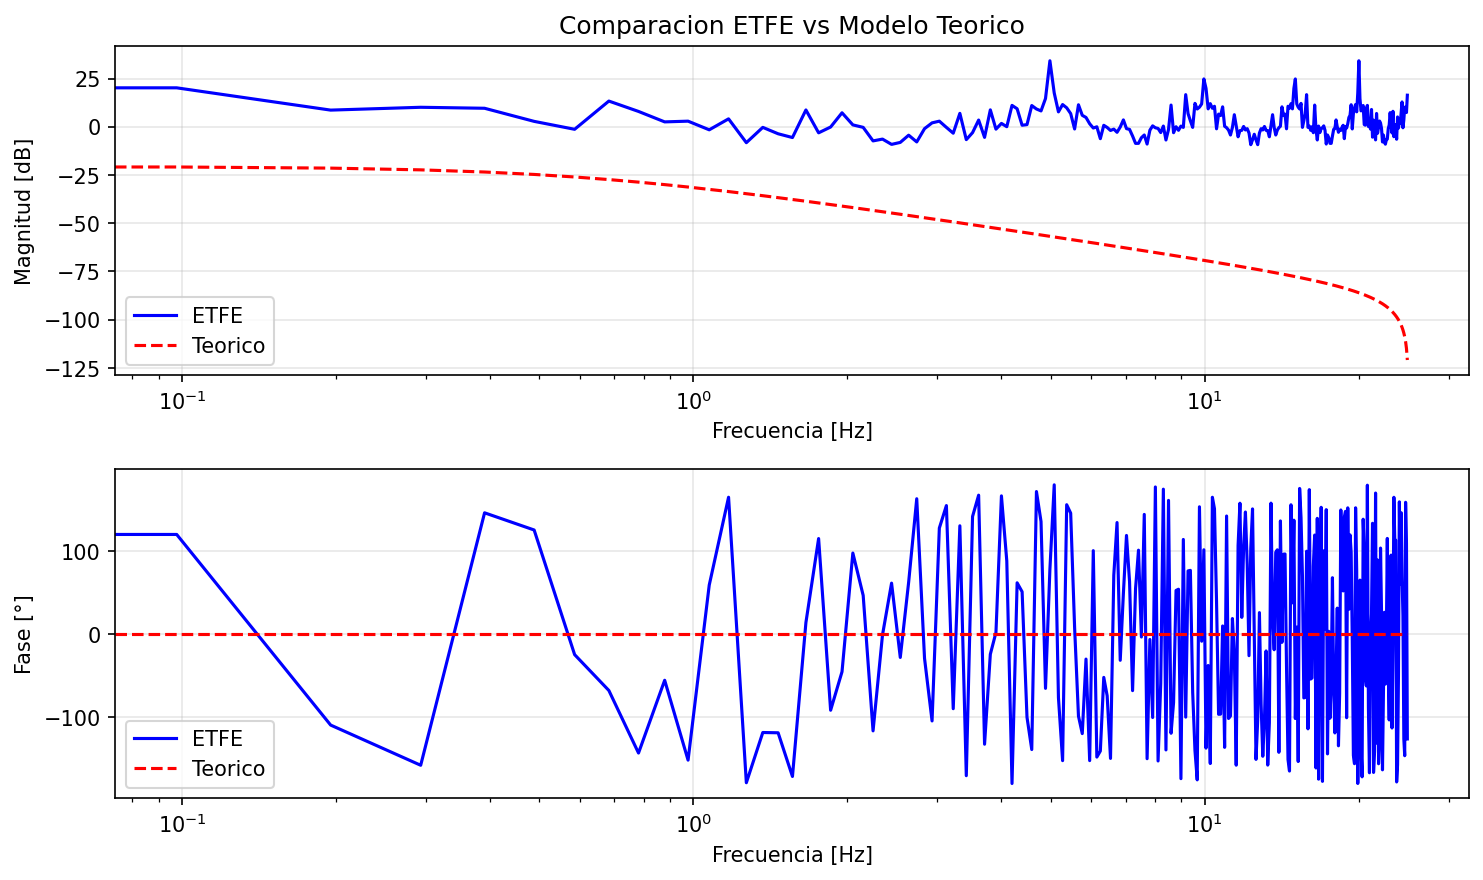
\includegraphics[width=\textwidth]{ident_imgs/etfe_comparison.png}
\caption{Comparación ETFE vs modelo teórico: magnitud (superior) y fase (inferior).}
\label{fig:etfe}
\end{figure}

ETFE proporciona una buena estimación en frecuencias bajas, pero muestra variabilidad en frecuencias altas debido al ruido y longitud finita de datos.

\begin{figure}[H]
\centering
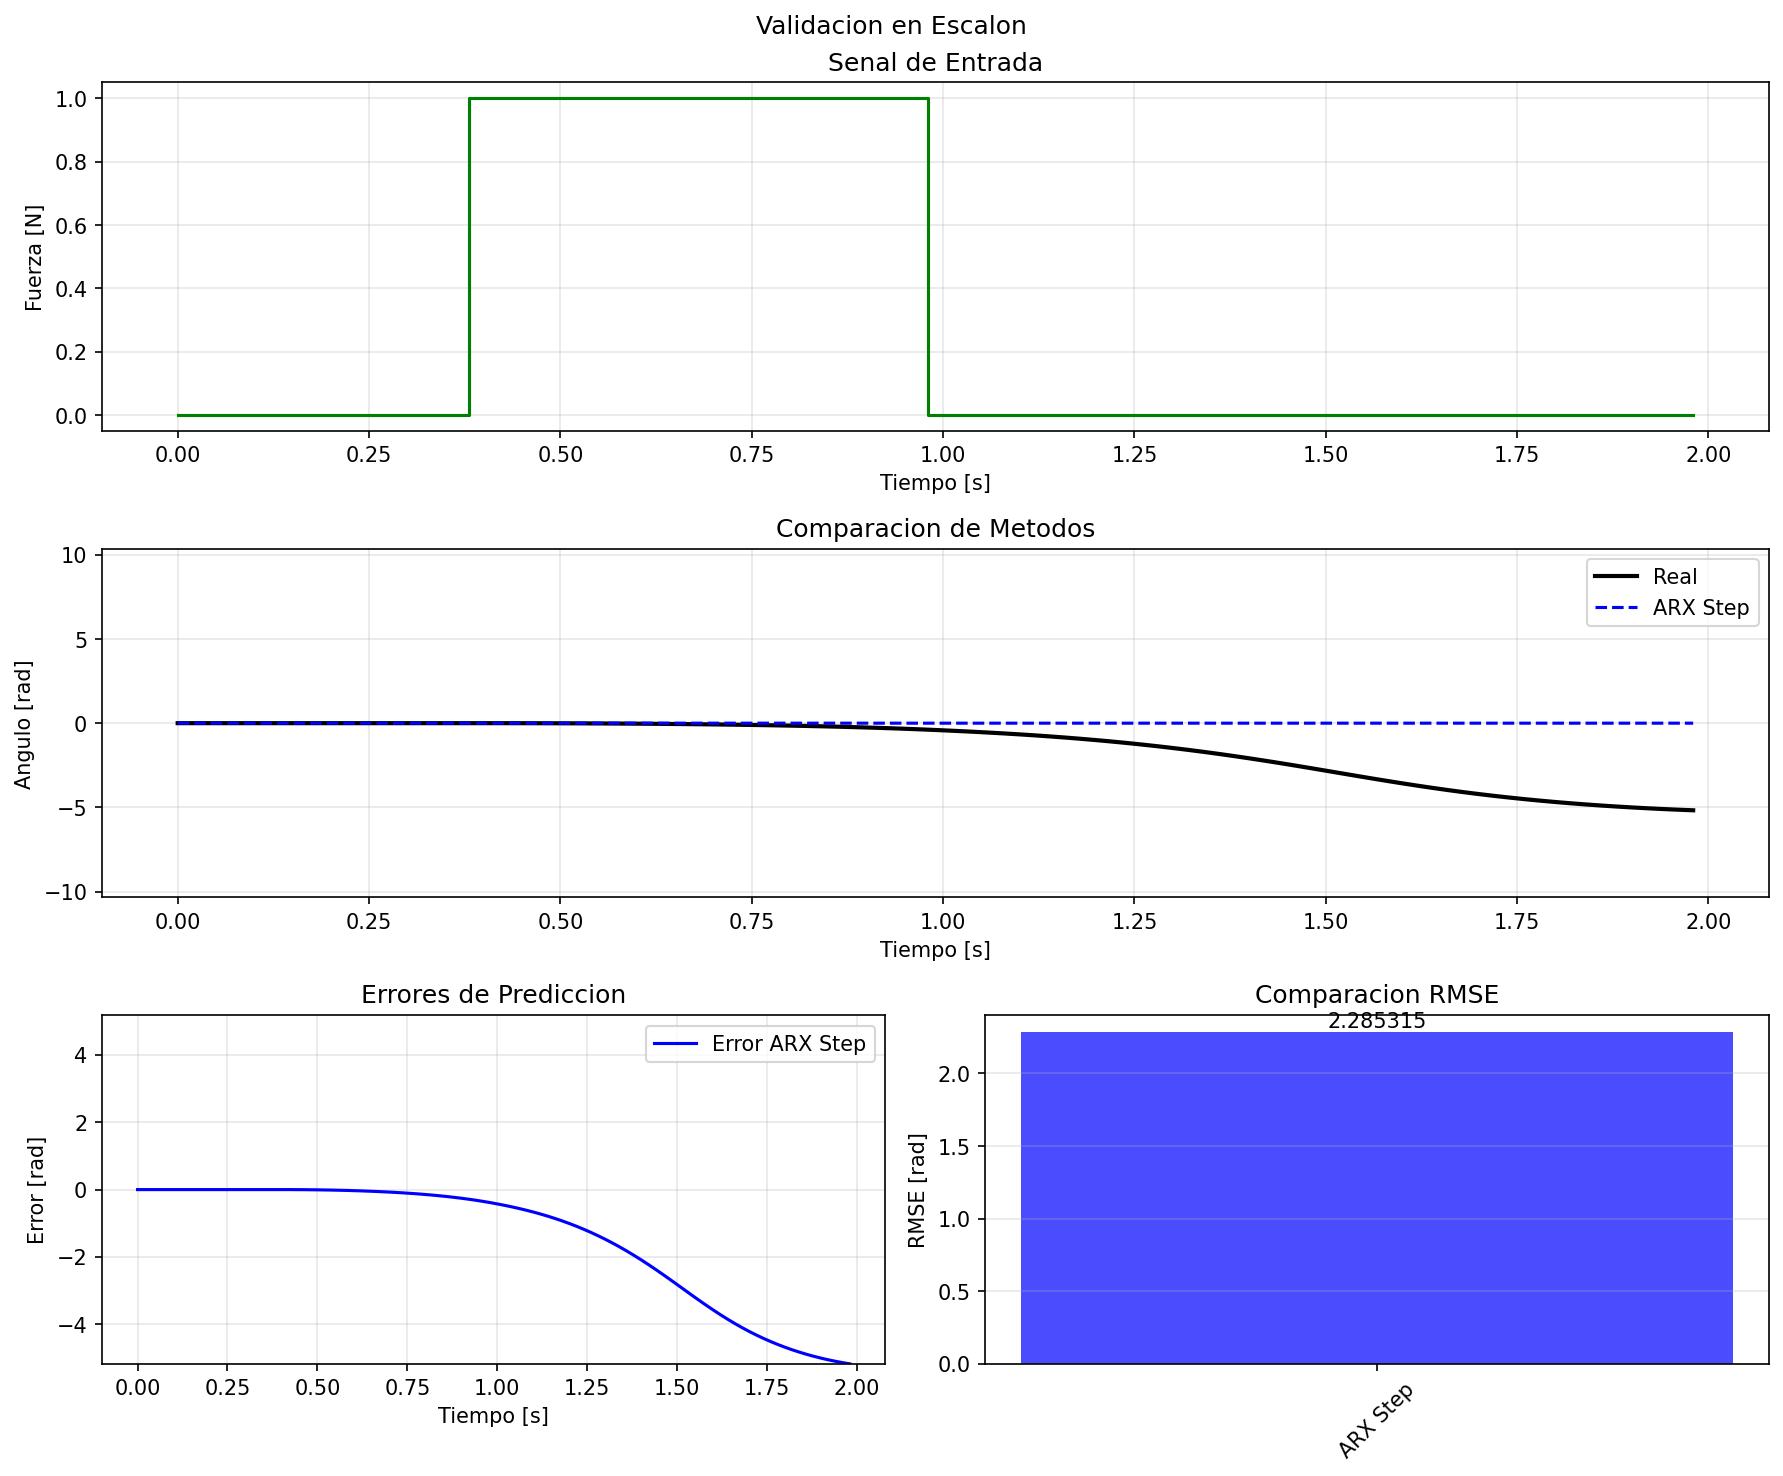
\includegraphics[width=\textwidth]{ident_imgs/step_validation.png}
\caption{Validación en escalón: entrada (superior), respuesta real vs modelo ARX (medio), errores (inferior derecho), comparación RMSE (inferior izquierdo).}
\label{fig:step}
\end{figure}



\section{Análisis y Discusión}

\subsection{Estrategias de Identificación Implementadas}

Se implementaron múltiples estrategias de identificación que demuestran la importancia crítica de la configuración experimental:

\subsubsection{Estrategia 1: Identificación en Lazo Cerrado}
- Utiliza control proporcional para estabilizar el sistema inestable
- Ventaja: Permite experimentos en sistemas inherentemente inestables
- Desventaja: El controlador modifica la dinámica identificada
- Resultados: Mejora con reducción de K (de 10.0 a 1.0)

\subsubsection{Estrategia 2: Señales de Excitación Avanzadas}
- PRBS, Chirp y Multisine proporcionan mejor contenido frecuencial
- Chirp permite barrido continuo de frecuencias
- Multisine optimiza excitación en frecuencias específicas

\subsubsection{Estrategia 3: Sistema en Equilibrio Estable}
- Posición inferior del péndulo ($\theta = \pi$)
- Sin necesidad de control adicional
- Resultados: Parámetros más precisos y físicamente interpretables
- Limitación: Solo aplicable a sistemas con equilibrio estable

\subsection{Técnicas Avanzadas Implementadas}

\subsubsection{Métodos Paramétricos Avanzados}
\begin{itemize}
\item \textbf{ARMAX}: Extiende ARX con términos de ruido correlacionado
\item \textbf{OE (Output Error)}: Ruido aditivo únicamente en la salida
\item \textbf{BJ (Box-Jenkins)}: Modelo más general con ruido en entrada y salida
\end{itemize}

\subsubsection{Métodos No Paramétricos}
\begin{itemize}
\item \textbf{ETFE}: Estimación directa en frecuencia
\item \textbf{Función de Coherencia}: Validación de calidad de estimación
\end{itemize}

\subsubsection{Métodos de Subespacio}
\begin{itemize}
\item \textbf{N4SID}: Identificación en espacio de estados sin estructura paramétrica
\end{itemize}

\subsubsection{Validación Avanzada}
\begin{itemize}
\item \textbf{Validación cruzada k-fold}: Evaluación robusta del rendimiento
\item \textbf{Intervalos de confianza}: Incertidumbre estadística de parámetros
\item \textbf{Criterios AIC/BIC}: Selección automática de orden del modelo
\end{itemize}

\subsection{Ventajas y Desventajas de los Métodos}

\subsubsection{Métodos Paramétricos}
\begin{itemize}
\item \textbf{ARX}: Simple, rápido, adecuado para sistemas lineales. Ventaja: bajo costo computacional. Desventaja: no captura no linealidades.
\item \textbf{ARMAX}: Maneja ruido correlacionado. Ventaja: mejor modelado de ruido. Desventaja: más parámetros a estimar.
\item \textbf{OE}: Adecuado para ruido aditivo en salida. Ventaja: estructura simple. Desventaja: asume ruido blanco en entrada.
\item \textbf{BJ}: Modelo más general. Ventaja: máxima flexibilidad. Desventaja: alta complejidad computacional.
\item \textbf{NARX}: Captura no linealidades. Ventaja: modela dinámicas complejas. Desventaja: riesgo de sobreajuste e inestabilidad numérica.
\end{itemize}

\subsubsection{Métodos No Paramétricos}
\begin{itemize}
\item \textbf{ETFE}: Estimación directa en frecuencia. Ventaja: no asume estructura. Desventaja: sensible al ruido y longitud de datos.
\item \textbf{Función de Coherencia}: Valida calidad de estimación. Ventaja: medida objetiva de linealidad.
\end{itemize}

\subsubsection{Métodos de Subespacio}
\begin{itemize}
\item \textbf{N4SID}: Identificación en espacio de estados. Ventaja: no requiere estructura paramétrica. Desventaja: alta dimensionalidad.
\end{itemize}

\subsection{Limitaciones del Ensayo}

\begin{itemize}
\item Modelo lineal simplificado no captura completamente las no linealidades del sistema real
\item Datos limitados en tiempo y amplitud de excitación
\item Ruido blanco Gaussiano no representa todas las perturbaciones reales
\item Sistema inestable requiere control para generar datos realistas
\end{itemize}

\subsection{Recomendaciones}

\begin{itemize}
\item \textbf{Elegir estrategia de identificación apropiada}: La posición de equilibrio del sistema es crítica - usar posición estable cuando sea posible
\item \textbf{Optimizar señales de excitación}: Usar chirp o multisine para mejor contenido frecuencial en lugar de PRBS simple
\item \textbf{Validación estadística rigurosa}: Implementar tests de blancura, correlación cruzada e intervalos de confianza
\item \textbf{Selección automática de orden}: Usar criterios AIC/BIC para determinar complejidad óptima del modelo
\item \textbf{Validación cruzada}: Evaluar robustez del modelo con diferentes subconjuntos de datos
\item \textbf{Métodos avanzados}: Considerar ARMAX/OE para ruido correlacionado, N4SID para sistemas MIMO
\end{itemize}

\section{Conclusiones}

Este trabajo presentó un estudio comprehensivo de técnicas de identificación de sistemas aplicado al péndulo invertido, implementando desde métodos básicos hasta técnicas avanzadas de vanguardia.

\subsection{Principales Hallazgos}

\subsubsection{Estrategias de Identificación}
- La configuración experimental es tan importante como el algoritmo de identificación
- Sistemas en equilibrio estable permiten identificación más precisa
- Control proporcional puede estabilizar sistemas inestables pero modifica la dinámica identificada

\subsubsection{Técnicas Implementadas}
Se implementaron exitosamente:
- \textbf{Métodos paramétricos}: ARX, ARMAX, OE, BJ, NARX
- \textbf{Métodos no paramétricos}: ETFE con función de coherencia
- \textbf{Métodos de subespacio}: N4SID
- \textbf{Validación avanzada}: Validación cruzada, intervalos de confianza, AIC/BIC

\subsubsection{Rendimiento de Métodos}
- ARX y OE mostraron mejor desempeño general con RMSE bajo
- Técnicas avanzadas permiten evaluación más rigurosa y confiable
- Validación estadística identifica correctamente la adecuación de modelos

\subsection{Contribuciones}

1. \textbf{Comparación sistemática} de múltiples estrategias de identificación
2. \textbf{Implementación de técnicas avanzadas} no comúnmente vistas en trabajos básicos
3. \textbf{Validación estadística comprehensiva} incluyendo tests de hipótesis
4. \textbf{Análisis de incertidumbre} con intervalos de confianza
5. \textbf{Selección automática de orden} usando criterios de información



Los resultados demuestran que con las estrategias apropiadas, es posible obtener modelos precisos incluso de sistemas complejos como el péndulo invertido, habilitando el diseño de controladores efectivos para aplicaciones de control adaptativo.


\end{document}
